\documentclass[titlepage]{article}
\usepackage[utf8]{inputenc}
\usepackage[T1]{fontenc}
\usepackage{graphicx}
\usepackage{caption} 
\usepackage{listings}
\usepackage{xcolor}
\usepackage{tabularx}
\usepackage{colortbl}

\title{Rapport MT10 - TP2 : Autour du RSA}
\author{Martin Schneider, Océane Bordeau}
\date{10 mai 2022}

\setlength{\parindent}{0pt}
\definecolor{codegreen}{rgb}{0,0.6,0}
\definecolor{codegray}{rgb}{0.5,0.5,0.5}
\definecolor{gray}{rgb}{0.8,0.8,0.8}
\definecolor{codepurple}{rgb}{0.58,0,0.82}
\definecolor{codeblue}{rgb}{0,0,255}
\definecolor{backcolour}{rgb}{0.95,0.95,0.92}

\lstdefinestyle{mystyle}{ 
    commentstyle=\color{magenta},
    keywordstyle=\color{codeblue},
    numberstyle=\tiny\color{codegray},
    stringstyle=\color{codepurple},
    basicstyle=\ttfamily\footnotesize,
    breakatwhitespace=false,         
    breaklines=true,                 
    captionpos=b,                    
    keepspaces=true,                                  
    showspaces=false,                
    showstringspaces=false,
    showtabs=false,                  
    tabsize=2
}

\lstset{style=mystyle}

\begin{document}
    \maketitle
    \tableofcontents
    \pagebreak

    \section{Préliminaire : \texttt{SageMath} et les nombres entiers}
    \textbf{Division euclidienne :}
    On utilise \texttt{divmod(x,y)} pour la division euclidienne de x par y, qui renvoie un couple $(div, mod)$ tel que :
    \[div*y + mod = x\]

    \begin{tabularx}{12cm}{|p{0.60cm}|X|}
        \hline
        \rowcolor{gray}
        \texttt{In}
        & 
        \texttt{divmod(15,4)}
        \\
        \hline
        \texttt{Out}
        &
        \texttt{(3,3)}
        \\
        \hline
    \end{tabularx}
    \bigbreak\bigbreak

    \textbf{Algorithme d'Euclide :}
    On utilise \texttt{gcd(a,b)} pour l'algorithme d'Euclide, qui renvoie le plus grand diviseur commun (PGCD) de a et b. \bigbreak

    \begin{tabularx}{12cm}{|p{0.60cm}|X|}
        \hline
        \rowcolor{gray}
        \texttt{In}
        & 
        \texttt{gcd(15,20)}
        \\
        \hline
        \texttt{Out}
        &
        \texttt{5}
        \\
        \hline
    \end{tabularx}
    \bigbreak\bigbreak

    \textbf{Algorithme d'Euclide étendu :}
    On utilise \texttt{xgcd(a,b)} pour l'algorithme d'Euclide étendu de a et b, qui renvoie un triple $(g, s, t)$ tel que :
    \[g = s*a + t*b = PGCD(a,b)\]

    \begin{tabularx}{12cm}{|p{0.60cm}|X|}
        \hline
        \rowcolor{gray}
        \texttt{In}
        & 
        \texttt{xgcd(15,20)}
        \\
        \hline
        \texttt{Out}
        &
        \texttt{(5,-1,-1)}
        \\
        \hline
    \end{tabularx}
    \bigbreak\bigbreak

    \textbf{Nombres premiers :} \bigbreak
    
    On utilise \texttt{is\_prime(x)} qui retourne \texttt{True} si le nombre est premier, \texttt{False} sinon. \bigbreak

    \begin{tabularx}{12cm}{|p{0.60cm}|X|}
        \hline
        \rowcolor{gray}
        \texttt{In}
        & 
        \texttt{is\_prime(15)}
        \\
        \hline
        \texttt{Out}
        &
        \texttt{False}
        \\
        \hline
    \end{tabularx}
    \bigbreak

    On utilise \texttt{prime\_range(x)} qui retourne la liste des nombres premiers strictement inférieurs à \texttt{x}. \bigbreak

    \begin{tabularx}{12cm}{|p{0.60cm}|X|}
        \hline
        \rowcolor{gray}
        \texttt{In}
        & 
        \texttt{prime\_range(15)}
        \\
        \hline
        \texttt{Out}
        &
        \texttt{[2, 3, 5, 7, 11, 13]}
        \\
        \hline
    \end{tabularx}
    \bigbreak

    On utilise \texttt{next\_prime(x)} qui retourne le premier nombre premier strictement supérieur à \texttt{x}. \bigbreak

    \begin{tabularx}{12cm}{|p{0.60cm}|X|}
        \hline
        \rowcolor{gray}
        \texttt{In}
        & 
        \texttt{next\_prime(17)}
        \\
        \hline
        \texttt{Out}
        &
        \texttt{19}
        \\
        \hline
    \end{tabularx}
    \bigbreak

    On utilise \texttt{factor(x)} qui retourne la décomposition de \texttt{x} en facteurs de nombres premiers. \bigbreak

    \begin{tabularx}{12cm}{|p{0.60cm}|X|}
        \hline
        \rowcolor{gray}
        \texttt{In}
        & 
        \texttt{factor(150)}
        \\
        \hline
        \texttt{Out}
        &
        \texttt{2 * 3 * 5$^ 2$ }
        \\
        \hline
    \end{tabularx}
    \bigbreak

    On utilise \texttt{prime\_pi(x)} qui compte combien de nombres premiers sont inférieurs où égaux à \texttt{x}. \bigbreak

    \begin{tabularx}{12cm}{|p{0.60cm}|X|}
        \hline
        \rowcolor{gray}
        \texttt{In}
        & 
        \texttt{prime\_pi(x)}
        \\
        \hline
        \texttt{Out}
        &
        \texttt{6}
        \\
        \hline
    \end{tabularx}
    \bigbreak

    \section{Nombres premiers}
    \subsection{Sur la répartition des nombres premiers}
    \bigbreak
    L’objectif est d’observer le comportement de suite $u_n = \pi(n)\frac{\ln n}{n}$, pour des n les plus grands possibles.
    \bigbreak
    1. Jusqu'à $10^{13}$, la commande \texttt{prime\_pi} met moins d'une dizaine de seconde à s'éxécuter, pour $10^{14}$, l'éxécution prend envirion 55 secondes. La limite de la minute est atteinte pour $10^{15}$.
    \bigbreak
    2. $\pi (n)$ désigne les nombres premiers $\leq n$.\newline
    Traçons sur un même graphique $n \mapsto \pi (n)$ et $n \mapsto \frac{n}{\ln n}$ :  
    \begin{center}
        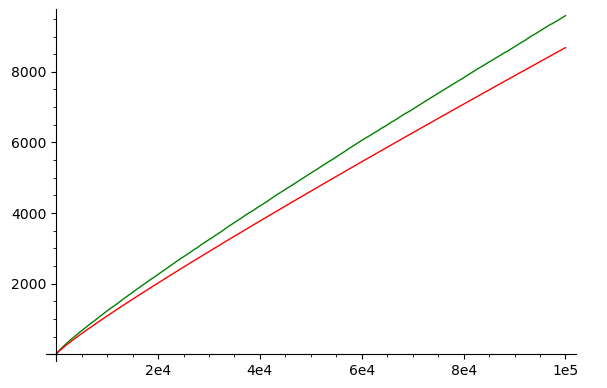
\includegraphics[scale=0.5]{Ressources/2022-04-27-10:20:27-screenshot.png}
        \captionof{figure}{}
        \end{center}
    \bigbreak
    3. Traçons $u_n$ en fonction de $n$ : 
    \begin{center}
        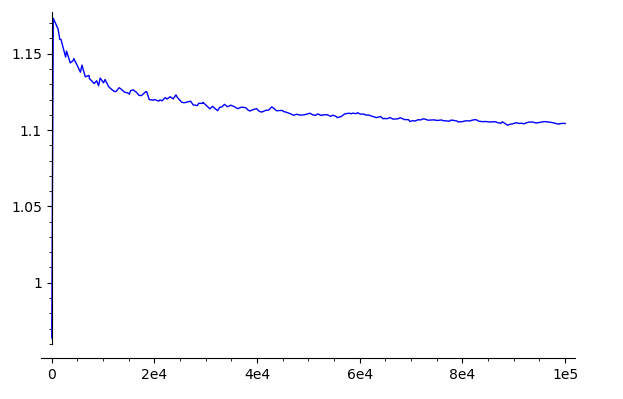
\includegraphics[scale=0.5]{Ressources/2022-04-27-10:20:31-screenshot.png}
        \captionof{figure}{}
    \end{center}
    Comme annoncé par le théorème des nombres premiers, la suite $u_n$ semble tendre vers $1$.
    \bigbreak

    \subsection{Nombres de Fermat}

    \subsection{Nombres de Mersenne}
    1. La liste des nombres premiers inférieurs ou égaux à 257 est la suivante, il y en a 55.\bigbreak
    \begin{tabularx}{12cm}{|p{0.60cm}|X|}
        \hline
        \rowcolor{gray}
        \texttt{In}
        & 
        \texttt{prime\_range(258)}
        \\
        \hline
        \texttt{Out}
        &
        \texttt{[2,3,5,7,11,13,17,19,23,29,31,37,41,43,47,53,59,61,67,71,\newline
        73,79,83,89,97,101,103,107,109,113,127,131,137,139,149,\newline
        151,157,163,167,173,179,181,191,193,197199,211,223,227,\newline
        229,233,239,241,251,257]}
        \\
        \hline
        \rowcolor{gray}
        \texttt{In}
        & 
        \texttt{prime\_pi(257)}
        \\
        \hline
        \texttt{Out}
        &
        \texttt{55}
        \\
        \hline
    \end{tabularx}
    \bigbreak
    On forme la liste des nombres de Mersenne correspondants.

    \lstinputlisting[language=Python, firstline=199, lastline=201]{sourceCode.py}

    2. Parmi la liste précédente, on affiche seulement les valeurs de $p$ pour lesquelles $M_p$ est premier :

    \lstinputlisting[language=Python, firstline=203, lastline=205]{sourceCode.py}

    \begin{tabularx}{12cm}{|p{0.60cm}|X|}
        \hline
        \texttt{Out}
        &
        \texttt{2,3,5,7,13,17,19,31,61,89,107,127}
        \\
        \hline
    \end{tabularx}
    \bigbreak

    Mersenne s'est trompé, $M_p$ n'est pas premier pour $p = 67, 257$, mais l'est pour $p = 61, 89, 107$.\bigbreak

    3. On décompose $M_{41}$ et $M_{47}$ en facteurs premiers.\bigbreak

    \begin{tabularx}{12cm}{|p{0.60cm}|X|}
        \hline
        \rowcolor{gray}
        \texttt{In}
        & 
        \texttt{factor(pow(2,41)-1)}
        \\
        \hline
        \texttt{Out}
        &
        \texttt{13367 * 164511353}
        \\
        \hline
        \rowcolor{gray}
        \texttt{In}
        & 
        \texttt{factor(pow(2,47)-1)}
        \\
        \hline
        \texttt{Out}
        &
        \texttt{2351 * 4513 * 13264529}
        \\
        \hline
    \end{tabularx}
    \bigbreak

    Euler s'est donc bien trompé, $M_{41}$ et $M_{47}$ ne sont pas premiers.\bigbreak

    4. Pour les nombres de Mersenne $M_p$ premiers inférieurs ou égaux à 257, on vérifie que $n = 2^{p-1}M_p$ est parfait grâce aux fonctions suivantes.
    \lstinputlisting[language=Python, firstline=208, lastline=219]{sourceCode.py}

    \begin{tabularx}{12cm}{|p{0.60cm}|X|}
        \hline
        \texttt{Out}
        &
        \texttt{Mp premier pour p = 2\newline
        parfait ? True\newline
        Mp premier pour p = 3\newline
        parfait ? True\newline
        Mp premier pour p = 5\newline
        parfait ? True\newline
        Mp premier pour p = 7\newline
        parfait ? True\newline
        Mp premier pour p = 13\newline
        parfait ? True\newline
        Mp premier pour p = 17\newline
        parfait ? True\newline
        Mp premier pour p = 19\newline
        parfait ? True\newline
        Mp premier pour p = 31\newline
        parfait ? True\newline
        Mp premier pour p = 61\newline
        parfait ? True\newline
        Mp premier pour p = 89\newline
        parfait ? True\newline
        Mp premier pour p = 107\newline
        parfait ? True\newline
        Mp premier pour p = 127\newline
        parfait ? True}
        \\
        \hline
    \end{tabularx}
    \bigbreak

    \subsection{Un test de primalité pour les nombres de Mersenne}

    \section{Algorithmes d'exponentiation}
    \subsection{Naïf itératif et naïf récursif}
    L'objectif est ici de promgramme un algorithme d'exponentiation, de manière naïve. D'abord de façon itérative, puis récursive.

    \lstinputlisting[language=Python, firstline=13, lastline=17]{sourceCode.py}

    \lstinputlisting[language=Python, firstline=19, lastline=21]{sourceCode.py}

    \subsection{Dichotomique itératif et dichotomique récursif}

    On peut largement optimiser ces algorithmes en utilisant \- les formules dichotomiques : 

    \lstinputlisting[language=Python, firstline=23, lastline=28]{sourceCode.py}

    \lstinputlisting[language=Python, firstline=221, lastline=231]{sourceCode.py}

    \subsection{Algorithme d'exponentiation modulaire}
    On adapte l'algorithme récursif prédécent pour calculer $x^n [N]$.

    \lstinputlisting[language=Python, firstline=30, lastline=35]{sourceCode.py}

    On compare avec \texttt{power\_mod} :\bigbreak

    \begin{tabularx}{12cm}{|p{0.60cm}|X|}
        \hline
        \rowcolor{gray}
        \texttt{In}
        & 
        \texttt{dicho\_rec\_mod(15,1550,2410)}
        \\
        \hline
        \texttt{Out}
        &
        \texttt{225}
        \\
        \hline
        \rowcolor{gray}
        \texttt{In}
        & 
        \texttt{power\_mod(15,1550,2410)}
        \\
        \hline
        \texttt{Out}
        &
        \texttt{225}
        \\
        \hline
    \end{tabularx}
    \bigbreak

    \section{Cryptosystème RSA}
    \subsection{Codage et décodage d'un message}
    La permière étape est de définir deux méthodes capables de traduire un message alphabétique en une suite d'entiers compris entre $0$ et $N-1$ (N étant le module de notre clé RSA).
    Pour cela, on crée la fonction \texttt{numerise()} qui convertit la chaîne alphabétique en une chaine binaire grâce au codage ASCII. Un caractère étant codé sur un octet, cette chaîne fait 8 fois la longuer de la chaîne initiale.
    Il s'agit ensuite de diviser cette chaine en "paquets" de bits dont la taille est à adapter en fonction de $N$.
    Pour que la valeurs des paquets ne dépasse pas $N-1$, la taille de ces dernier ne peut pas dépasser $ln(N)/ln(2)$. Pour un soucis d'intégrité de la transformation, on va chercher la taille la plus grande, inférieur à $ln(N)/ln(2)$, et qui divise la longueur de la chaine binaire obtenue.
    Ainsi, tous les paquets auront la même taille. On utilise pour cela la fonction \texttt{chooseSize()} qui renvoie la taille idéale des paquets.
    Une fois la chaine de bits divisée, il suffit de retraduire ces paquets de bits en entier (qui par construction seront inférieurs à $N-1$).
    La fonction retourne alors un object \texttt{list} contenant les entiers recherchés.

    \lstinputlisting[language=Python, firstline=42, lastline=52]{sourceCode.py}

    La fonction \texttt{alphabetise()} effectue simplement le processus inverse.
    
    \lstinputlisting[language=Python, firstline=60, lastline=69]{sourceCode.py}

    Dans chaque fonction, certaines rectifications sont nécéssaires pour assurer la bijectivité de l'encodage et l'intégrité du message codé. Par exemple, nous avons définit notre propre fonctioon \texttt{toBin()}, plus sûre que la fonction \texttt{bin()} de la librairie Python. 

    \subsection{Génération de clés RSA}
    Pour la génération des clés, on définit la fonction \texttt{cleRSA()}. Cette dernière fait appel à différentes fonction pour définir les nombres $p$, $q$, $e$, et calculer $d$.

    \lstinputlisting[language=Python, firstline=71, lastline=102]{sourceCode.py}

    \subsection{Fonctions de chiffrement et déchiffrement RSA}

    \subsection{Signature avec RSA}
    \subsubsection{Protocole 1}
    \subsubsection{Protocole 2}

    \section{Factorisation de clefs RSA}
    Pour chercher une factorisation d'une clé RSA, le programme suivant suit la méthode de Fermat modifiée pour factoriser $N = pq$.
    On cherche une écriture du type $LN = R^2 - S^2$ où $L,R,S$ sont des entiers positifs tels que $L$ et $S$ petits.
    Si cette écriture existe, on peut trouver les facteurs $p$ et $q$ (non triviaux) en calculant $pgcd(N,R-S)$ et $ pgcd(N,R+S)$.

    \lstinputlisting[language=Python, firstline=121, lastline=137]{sourceCode.py}

    Pour des clés RSA relativement petites, on trouve rapidement la factorisation comme le montre l'exemple ci-dessous avec une clé RSA de 50 bits. \bigbreak

    \begin{tabularx}{12cm}{|p{0.60cm}|X|}
        \hline
        \rowcolor{gray}
        \texttt{In}
        & 
        \texttt{factorisationRSA(645150365822089)}
        \\
        \hline
        \texttt{Out}
        &
        \texttt{PCGD(N,R-S) =  24552379 \newline
        PGCD(N,R+S) =  26276491}
        \\
        \hline
    \end{tabularx}
    \bigbreak
    
    Si cette écriture du type $LN = R^2 - S^2$ existe, on dit que $N$ est périlleux, on peut bien évidemment trouver des clés RSA non périlleuses comme celle ci-dessous avec une clé de longueur 500 bits.\bigbreak
    
    \begin{tabularx}{12cm}{|p{0.60cm}|X|}
        \hline
        \rowcolor{gray}
        \texttt{In}
        & 
        \texttt{factorisationRSA(103077048898751646811845904379690253}
        \texttt{91827158046114929907021555374862351383356881742893451}
        \texttt{03743257562103172714870402164525935411301652888244783}
        \texttt{0478777256189)}
        \\
        \hline
        \texttt{Out}
        &
        \texttt{PCGD(N,R-S) =  1 \newline
        PGCD(N,R+S) =  1}
        \\
        \hline
    \end{tabularx}
    \bigbreak
    

    \section{Test de primalité probabilistes}
    On sait d'après le petit théorème de Fermat que si on trouve un entier $a \in \lbrack1,n-1\rbrack$
    tel que $a^{n-1} \neq 1 \lbrack n \rbrack$ alors on est sûr que $n$ n'est pas premier. 
    Le programme suivant tire aléatoirement $l$ valeurs (donné en paramètres) de $a$, 
    si le test de Fermat échoue alors $n$ est composé, et s'il réussit alors $n$ est premier ou de Carmichaël.

    \lstinputlisting[language=Python, firstline=139, lastline=144]{sourceCode.py}

    On choisit aléatoirement $l$ valeurs de $a$, si le test de Fermat échoue sur une de ces valeurs de $a$ alors
    $n$ est composé. Pour un nombre de Carmichaël $n$, plus on choisit un $l$ élevé, plus on a de chance que le test
    de Fermat échoue et nous renvoie que $n$ est composé, car il suffit que le test échoue une seule fois sur les $l$ 
    valeurs de $a$. \bigbreak
    Par exemple : \bigbreak

    \begin{tabularx}{12cm}{|p{0.60cm}|X|}
        \hline
        \rowcolor{gray}
        \texttt{In}
        & 
        \texttt{testPrimaliteFermat(2316845,200)}
        \\
        \hline
        \texttt{Out}
        &
        \texttt{False}
        \\
        \hline
        \rowcolor{gray}
        \texttt{In}
        & 
        \texttt{is\_prime(2316845)}
        \\
        \hline
        \texttt{Out}
        &
        \texttt{False}
        \\
        \hline
    \end{tabularx}
    \bigbreak

    Le plus petit entier composé qui passe le test de Fermat est 561, le plus petit entier de Carmichaël.
    Pour 2 valeurs de $a$, 561 passe presque immédiatement le test de Fermat mais pour 5 valeurs de $a$, 
    de temps en temps 561 ne passe pas le test de Fermat et nous renvoie $False$ car il suffit qu'une seule
    des 5 valeurs échoue le test de Fermat pour que la fonction nous renvoie $False$. Mais comme ces $a$
    sont aléatoires, parfois 561 réussit à passer le test.\newline

    On améliore le test avec le critère de Miller-Rabin.

    \lstinputlisting[language=Python, firstline=146, lastline=166]{sourceCode.py}

    Cette fois-ci 561 ne passe pas le test de Miller-Rabin : \bigbreak

    \begin{tabularx}{12cm}{|p{0.60cm}|X|}
        \hline
        \rowcolor{gray}
        \texttt{In}
        & 
        \texttt{testPrimaliteFermat(561,5)}
        \\
        \hline
        \texttt{Out}
        &
        \texttt{True}
        \\
        \hline
        \rowcolor{gray}
        \texttt{In}
        & 
        \texttt{is\_prime(561)}
        \\
        \hline
        \texttt{Out}
        &
        \texttt{False}
        \\
        \hline
        \rowcolor{gray}
        \texttt{In}
        & 
        \texttt{testPrimaliteMillerRabin(561,5)}
        \\
        \hline
        \texttt{Out}
        &
        \texttt{False}
        \\
        \hline
        
    \end{tabularx}
    \bigbreak

    Pour 5 valeurs de $a$, nous n'avons pas trouvé de nombre de Carmichaël qui passe le test de Miller-Rabin.

\end{document}
